\documentclass[a4paper, twoside, utf8]{ctexart}
\usepackage[fontset=Fandol]{ctex}
\usepackage{anyfontsize}
\usepackage{subcaption}
\usepackage{adjustbox}
\usepackage{algorithm}
\usepackage{longtable}
\usepackage{abstract}
\usepackage{amsfonts}
\usepackage{appendix}
\usepackage{booktabs}
\usepackage{enumitem}
\usepackage{fancyhdr}
\usepackage{geometry}
\usepackage{graphicx}
\usepackage{tabularx}
\usepackage{listings}
\usepackage{amsmath}
\usepackage{caption}
\usepackage{lipsum}
\usepackage{minted}
\usepackage{xcolor}
\usepackage{array}
\usepackage{url}

\geometry{a4paper,left=31mm,right=31mm,top=25mm,bottom=25mm}
\setlength{\parindent}{2em}
\ctexset{section = {format = \raggedright\large\bfseries}}
\let\oldsection\section
\renewcommand{\abstracttextfont}{\normalsize}

\pagestyle{fancy}
\fancyhf{}
\fancyhead[CO,CE]{后缀表达式 \ Postfix}
\fancyhead[LE]{编译器构造实验}
\fancyhead[RO]{Lab03实验报告}
\fancyhead[RE,LO]{}
\fancyfoot[CO]{\thepage}
\fancyfoot[CE]{\thepage}
\fancyfoot[LE,RE]{}
\fancyfoot[LO,RO]{}

\title{\songti \bfseries 后缀表达式 \ 实验报告}
\author{\fangsong 傅祉珏 \ \ 21307210}
\date{\fangsong 中山大学计算机学院\ 广东广州\ 510006}

\begin{document}
	
	\begin{titlepage}
		\centering
		\rule{\textwidth}{1pt}
		\vspace{0.02\textheight}
		
		{\LARGE \kaishu 编译器构造实验 \quad Lab03实验报告}
		
		\vspace{0.02\textheight}
		
		{\Huge \songti \bfseries 后缀表达式}
		
        \vspace{0.025\textheight}
        \rule{0.83\textwidth}{0.4pt}
        \vspace{0.05\textheight} 
        
        \begin{figure}[htbp]
            \centering
            
\includegraphics[width=8cm, height=8cm]{./figure/计院院徽.jpg}
        \end{figure}

        \vspace{0.05\textheight} 
        {\Large 课程编号:\textsc{DCS292}}

        \vspace{0.025\textheight} 
        {\Large 学生姓名:\textsc{傅祉珏}}

        \vspace{0.025\textheight} 
        {\Large 学生学号:\textsc{21307210}}

        \vspace{0.025\textheight} 
        {\Large 指导老师:\textsc{李文军\ 教授}}
 
        \vspace{0.025\textheight} 
        {\Large 项目截止日期:\textsc{2025年4月24日}}

        \vspace{0.05\textheight} 
        \vfill

        {\large \today}
        \vspace{0.1\textheight}
        \rule{\textwidth}{1pt}
    \end{titlepage}
	
    \pagenumbering{Roman}
    \setcounter{page}{1}
    \renewcommand{\abstractname}{\Large \textbf{引言}}
    \addcontentsline{toc}{section}{引言}
    \begin{abstract}
        编译器构造是计算机科学中的核心课程之一,其教学目标不仅在于传授理论知识,更强调通过实践活动加深对语言处理机制的理解。为此,课程设置了多个层次递进的实验任务,覆盖从词法分析、语法分析到语义翻译和中间代码生成的完整流程。本实验(Lab03)作为首次综合性实践任务,标志着从预备实验阶段过渡到编译器前端模块的深入探索。

        实验围绕“中缀表达式转后缀表达式”的语法制导翻译任务展开,选取《编译原理(第二版)》第二章所附的简化 Java 示例程序作为基础。原始程序基于递归下降方法实现,能够接受由数字($0\sim9$)和加减运算符构成的无空格中缀表达式,并输出其对应的后缀表达式。尽管该程序能正确运行,但在结构设计、错误处理和运行效率等方面仍存在明显不足,亟需优化和扩展。
        
        为提升程序的健壮性、可维护性与工程实用性,实验提出了以下改进目标:将程序中的静态成员重构为非静态成员,提升模块化水平;对原始递归结构进行尾递归消除,以提升执行性能并降低调用栈压力;引入更为完善的错误检测与恢复机制,增强容错能力;补充程序文档说明,使用 javadoc 工具生成标准化 API 文档;设计覆盖广泛的测试用例并使用 JUnit 框架进行单元测试,确保功能正确性和鲁棒性。
        
        通过结构优化和功能增强,该实验旨在构建一个具备良好工程规范、错误提示能力强、测试体系完备的中缀表达式转换工具,为后续语义分析及中间代码生成等模块的实现提供坚实基础。
        
        \vspace{1em}
        \noindent{\textbf{\heiti 关键词:}编译器构造;语法制导翻译;后缀表达式;尾递归优化;错误处理;JUnit 测试;文档生成。}
    \end{abstract}
    \newpage

    \addcontentsline{toc}{section}{目录}
    \begingroup
    \setcounter{tocdepth}{2}
    \renewcommand{\section}{
        \renewcommand{\raggedright}{}
        \ctexset{section/format = \centering\Large\bfseries}
        \oldsection
    }
    \tableofcontents
    \endgroup
    \newpage

    \pagenumbering{arabic}
    \setcounter{page}{1}
	
	\maketitle

    \section{项目概况}

    \subsection{项目背景}

    在完成了旨在帮助掌握 Java 语言开发流程与面向对象设计理念的预备实验之后,本实验作为编译原理课程中的首次综合性实践,标志着编译器构造学习的实质性开始。实验以改进一个简化的语言处理程序为核心任务,通过实践操作使参与者能够建立起对语言处理基本机制的初步理解,并进一步加深对《编译原理》(第二版,俗称“龙书”)第二章 A Simple Syntax-Directed Translator 所涉及内容的掌握。

    该章内容提供了一个完整的 Java 示例程序,其处理对象为一种结构简单的中缀表达式语言。该语言的运算元限定为 0 至 9 之间的单个数字,支持的运算符仅包括加法与减法,且不允许表达式中包含空格、制表符等空白符。程序的功能相对单一,核心任务是将用户输入的中缀表达式转换为等价的后缀表达式并输出。然而,当用户输入不符合语法规范时,程序不会提示错误信息,而是输出不可预测的结果。

    为便于开展实验,配套文档不仅提供了上述程序的完整源代码,还构建了一个简洁的实验环境,使参与者能够专注于程序结构理解与功能拓展。本实验的设置为后续深入掌握编译器前端的词法分析、语法分析及语义翻译等环节打下了基础,同时提升了对语法制导翻译技术实现细节的理解与运用能力。

    \subsection{实验需求}

    本实验旨在通过对实验平台所提供的中缀转后缀表达式转换程序进行结构性优化与功能拓展,深入理解编译器前端语法分析过程中的基本构件与实现方式。实验任务涵盖语法制导翻译、程序结构重构、错误处理机制设计、文档化规范与程序测试方法,具有较强的系统性与实践指导意义。

    实验的首要任务是分析原程序中 \verb|Parser| 类的静态成员变量 \verb|lookahead| 的设计合理性,并尝试将其重构为非静态成员变量,从而考察该修改对程序行为与逻辑正确性的影响。此过程可用于加深对 Java 编程语言中静态与非静态成员在类加载、内存模型及对象作用域管理中的差异理解,促进对语法分析器中状态管理机制的掌握。
    
    在性能优化方面,实验要求将原程序中的尾递归方法 \verb|rest()| 改写为等价的非递归迭代结构。尾递归虽然在逻辑表达上简洁明晰,但在执行效率与栈空间利用方面存在一定的局限性。通过消除尾递归并采用迭代方式实现语法分析逻辑,可提升程序执行效率,符合编译器优化中控制流转换的基本原则。
    
    程序的健壮性改进是实验中的另一重点。实验初始代码未对非法输入进行处理,缺乏基本的错误提示功能,导致程序在面对语法不合法表达式时可能产生无意义输出或异常行为。因此,有必要为程序添加完善的错误处理机制,能够在输入表达式存在词法或语法错误时给出明确的报错信息。更进一步,实验还鼓励实现错误的定位与分类提示,甚至在能力允许的前提下探索出错恢复策略,使程序在发现异常后仍能继续处理剩余部分,提升系统的容错能力和用户交互体验。
    
    实验同时强调编程规范与文档化的重要性。要求在源代码中添加符合 Java 编码规范的文档化注释,并利用 JDK 提供的 \verb|javadoc| 工具生成 HTML 格式的程序文档,统一保存在 \verb|doc| 目录中。该任务旨在培养良好的软件开发文档撰写习惯,提升代码可维护性和可读性,并为团队协作或后续开发提供支持。
    
    作为进阶任务,实验还鼓励使用 JUnit 等主流 Java 单元测试框架对改进后的程序进行系统性测试。通过构造覆盖全面的测试用例,可有效验证各功能模块在不同输入条件下的稳定性与正确性,进一步增强程序的可靠性,并促进对测试驱动开发(TDD)理念与实践方法的理解。

    \section{语法分析}

    \subsection{源代码分析}

    该程序的核心任务是将中缀表达式转换为后缀表达式。为了完成这一任务,程序实现了递归下降解析器(Recursive Descent Parser),并通过逐步解析输入的中缀表达式来生成等价的后缀表达式。为了更好地理解源代码的实现,需要先明确该程序处理的语法结构。源代码可见\textit{附录A:原始源程序清单}。

    程序中所处理的语法基于简单的算术表达式,其文法规则可表示为:

    \begin{equation}
        \begin{aligned}
            \texttt{expr} \quad & ::= \quad \texttt{term} \ \texttt{rest} \\
            \texttt{rest} \quad & ::= \quad + \ \texttt{term} \ \texttt{rest} \quad | \quad - \ \texttt{term} \ \texttt{rest} \quad | \quad \varepsilon \\
            \texttt{term} \quad & ::=  \quad \texttt{digit} \\
        \end{aligned}
    \end{equation}
    \vspace{.5em}
    
    在该文法中,\verb|expr|是一个表达式,表示由一个 \verb|term|(操作数)后跟零个或多个加法或减法操作构成的表达式。\verb|rest| 代表一个可能的加法或减法操作的扩展,其中 $\varepsilon$ 表示空串,意味着当没有加法或减法操作时,表达式解析结束。\verb|term| 则表示一个数字,程序仅支持操作数为单个数字的算式(数字 0 到 9),这是该程序的一个局限性。

    源代码的语法分析过程严格按照这一文法进行。具体来说,\verb|Parser| 类中的 \verb|expr()| 方法对应于文法中的 \verb|expr|,其实现首先调用 \verb|term()| 方法来处理操作数。\verb|term()| 方法识别单个数字,并将其输出至标准输出流,同时继续读取下一个字符。接下来,\verb|expr()| 调用 \verb|rest()| 方法,用于处理加法和减法操作符的递归调用,直到没有更多的运算符为止,从而完成表达式的解析。

    在 \verb|rest()| 方法中,当遇到加号 $+$ 或减号 $-$ 时,程序通过调用 \verb|match()| 方法来匹配当前的运算符,并随后调用 \verb|term()| 方法继续处理下一个数字。在识别到运算符后,程序会将其输出至标准输出流,以此构建后缀表达式。在没有遇到加号或减号时,\verb|rest()| 方法返回,不再继续处理,从而结束了当前表达式的解析。

    \verb|term()| 方法用于处理中缀表达式中的数字。它首先检查当前字符是否为数字(通过 \verb|Character.isDigit()| 判断),若是数字,则将其输出并调用 \verb|match()| 方法更新 \verb|lookahead|,否则抛出语法错误。这确保了程序只能处理有效的数字字符。

    该程序的语法结构较为简单,主要通过递归下降的方式将输入的中缀表达式按文法规则转化为后缀表达式。程序中的 \verb|lookahead| 变量用作前瞻符号,控制程序的语法分析过程。它存储当前读取的字符,帮助判断是否匹配当前预期的运算符或操作数。程序通过不断读取字符并调用相应的匹配函数(\verb|match()|),逐步推进分析过程。

    然而,该程序假设输入的中缀表达式是有效的,并未对非法输入进行详细的错误处理。当遇到无效字符或不符合预期的表达式结构时,程序会抛出语法错误,这限制了程序的健壮性。为提高程序的容错性,后续可以通过引入更复杂的语法分析方法(如 LL 分析或 LR 分析)和错误恢复机制来增强程序的错误检测与修复能力。此外,尾递归优化也是该程序的潜在改进方向,特别是在 \verb|rest()| 方法的递归调用部分,可以通过转换为循环的方式提高程序的执行效率,避免递归深度过大时可能导致的栈溢出问题。

    \subsection{递归消除}

    在本实验所使用的表达式文法中,尾递归的形式清晰地体现在 \verb|rest| 的定义中。该非终结符在其递归产生式中以自身结尾,构成典型的尾递归结构。为了实现高效的自顶向下语法分析,并避免函数栈的多次递归开销,有必要将此类尾递归形式进行改写,使之适合以循环结构实现。尾递归的消除并不改变原有文法所定义语言的语义,只是将递归过程转换为等价的迭代过程,从而提升解析器执行的稳定性和性能。

    具体而言,尾递归的消除可通过将递归分支改写为在主函数体内使用的循环语句完成。在处理 \verb|expr| 时,首先识别一个 \verb|term|,之后进入一个循环结构,循环判断当前的 \verb|lookahead| 是否为 $+$ 或 $-$。若匹配到这些运算符之一,则继续读取一个 \verb|term| 并在逻辑结构中将其与之前的中间结果结合;若未匹配,则说明不再存在递归情况,循环终止。这样的转换逻辑等价于原有的尾递归定义,但避免了函数自身的多次调用与返回,使语法分析器更适合处理较长表达式或嵌套较深的输入。

    \begin{equation}
        \begin{aligned}
            \texttt{expr} \quad & ::= \quad \texttt{term} \ (+ \ | \ -) \ \texttt{term} \quad | \quad \texttt{term} \\
            \texttt{term} \quad & ::=  \quad \texttt{digit} \\
        \end{aligned}
    \end{equation}
    \vspace{.5em}
    
    这种自顶向下分析中尾递归的迭代重写方式与状态转换图的建模思想是一致的。在状态图中,进入 \verb|rest| 状态后,根据当前输入符号分支转向 $+$ 或 $-$ 的对应路径,然后回到 \verb|rest| 的起点状态,这一过程可通过状态的回边来模拟循环结构。在分析器设计中,利用循环控制逻辑实现这样的“回边”状态跳转,使得语法分析能够在不增加函数调用深度的情况下重复处理多个操作符与操作数,从而高效地解析完整的表达式序列。尾递归的消除不仅符合 TopDownParsing 所需的可预测输入处理顺序,也为表达式求值或转换的后续处理提供了清晰的中间结构。

    \begin{figure}
        \centering
        \begin{minipage}{.45\textwidth}
            \centering
            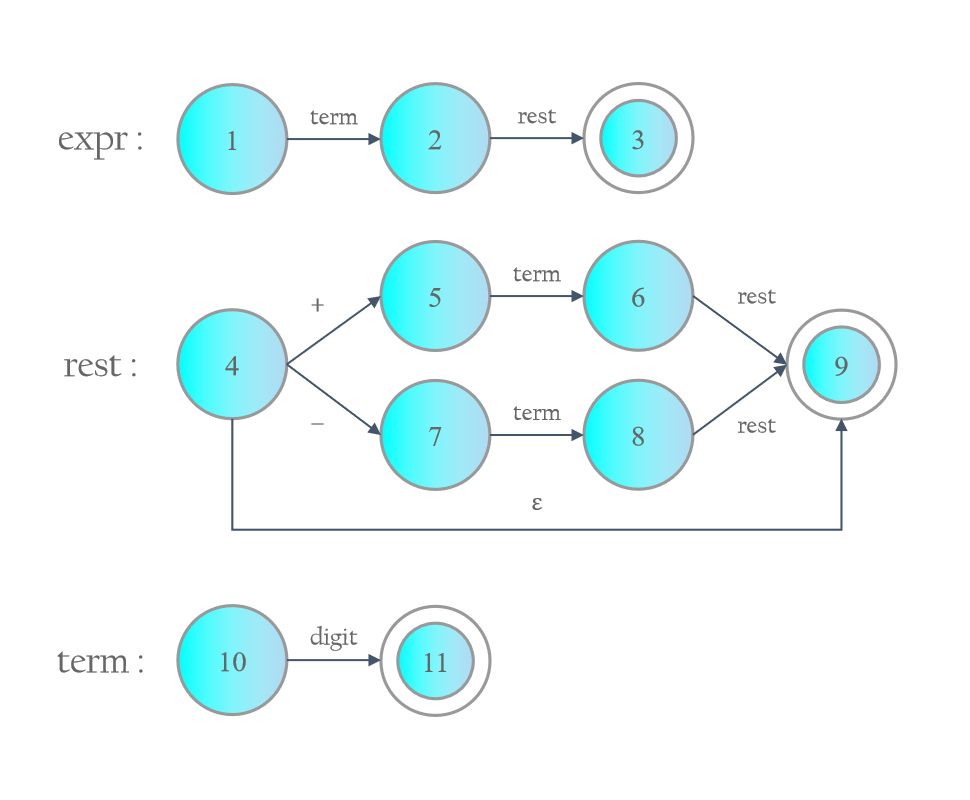
\includegraphics[width=.9\textwidth]{figure/TD.png}
            \caption{原文法状态转换图}
        \end{minipage}
        \begin{minipage}{.45\textwidth}
            \centering
            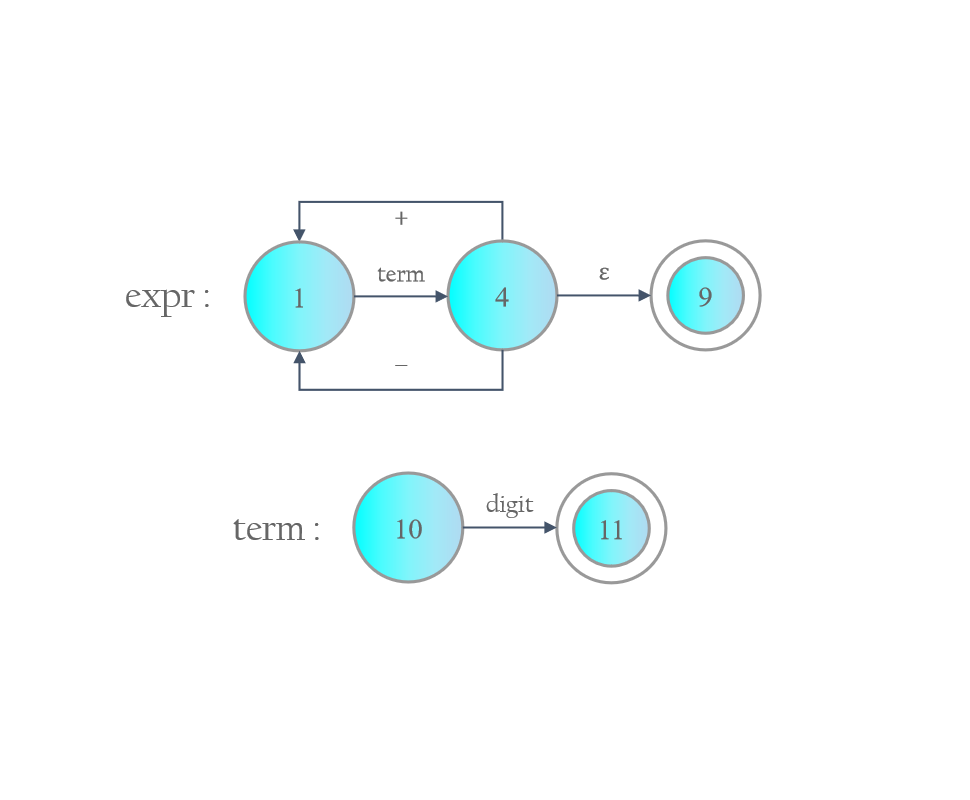
\includegraphics[width=.9\textwidth]{figure/RTD.png}
            \caption{约简文法状态转换图}
        \end{minipage}
    \end{figure}

    \subsection{异常处理}

    在本实验所设计的语法分析过程中,错误处理机制不仅保障了程序在面对不符合文法的输入时的稳定性与可控性,同时也通过明确的分类处理,覆盖了可能出现的多种典型语法错误类型。整个错误识别与恢复流程建立在自顶向下分析模型的基础上,通过持续监测当前输入符号(lookahead)与期望符号之间的一致性,在检测到偏差时迅速作出反应。

    具体而言,该语法分析器针对以下几类错误进行了处理与提示:首先是非法符号错误,即在期望读取数字或合法运算符时,遇到了诸如 $*$、$/$、$($ 或 $)$ 等未在当前文法中定义的符号,此类符号在实验设定的简化表达式语言中并无语义支持,因此一旦出现便立即触发错误提示。其次是空格误用错误,实验所使用的分析器并未设计跳过空格或对其进行预处理,因此空格在表达式的任何结构性位置上出现均被视为非法输入。这类设计虽然较为严格,但有助于强调对语法结构严谨性的要求,并迫使用户遵循明确的格式标准。

    第三类是多位数字错误,这是一种源于文法层级约束的特定错误类型。尽管在一般表达式处理系统中多位数字被认为是合法的常数项,但本实验中的语法仅定义了 $\texttt{term} \rightarrow \texttt{digit}$,即一个合法的项仅由单个数字组成。因此,当系统识别到连续数字字符构成的数值时,会主动检测其长度,若超过一位,便视为违背文法的结构性错误,并给出相应位置的详细提示。

    最后,是匹配失败错误,当语法分析器尝试匹配某个运算符或项的预期字符时,如果当前符号与预期符号不符,便立即触发错误报告,指出期望与实际之间的不一致,并中止当前分析过程。值得注意的是,在整个错误处理机制中,为每种错误情况配备了明确的提示信息和视觉输出标识(如输出标记为 \verb|(error)|),使得用户不仅能够获知存在语法错误,还能直观地定位其在表达式中的具体位置。

    通过上述这些错误类型的识别与处理,语法分析器在保持整体结构简洁明晰的同时,成功地实现了对于非法输入的基本语义隔离与控制,为实验教学场景中的表达式解析任务提供了良好的错误容忍性和交互反馈体验。

    \section{实验分析}

    \subsection{功能性案例测试}

    为验证语法分析器在表达式转换功能上的正确性,本实验针对多个代表性输入构造了功能性测试用例,覆盖基础加法、加减混合运算及长串嵌套运算等典型情形。测试方法采用将标准输入流重定向为模拟输入,并捕获标准输出流以获取后缀表达式的转换结果,进而与期望输出进行比对验证。所有测试均通过 JUnit 框架实现,确保了自动化测试的稳定性与重复性。

    测试样例包括 “$1+1$”、“$9-5+2$”、“$1+2+3+4+5$” 以及 “$1-2+3-4+5-6+7-8+9-0$” 等多组不同长度与运算复杂度的表达式。从转换结果来看,分析器能够正确地将中缀表达式转换为对应的后缀表达式。例如,“$1+1$” 被成功转换为 “$1 1 +$”,而较长的表达式 “$1-2+3-4+5-6+7-8+9-0$” 则被准确地转换为 “$1 2 - 3 + 4 - 5 + 6 - 7 + 8 - 9 + 0 -$”。这一结果表明,该程序已较为全面地实现了实验目标中的表达式识别与运算顺序处理能力,特别是在操作符优先级、结合性等关键规则的实现上表现稳定。

    \begin{figure}[htbp]
        \centering
        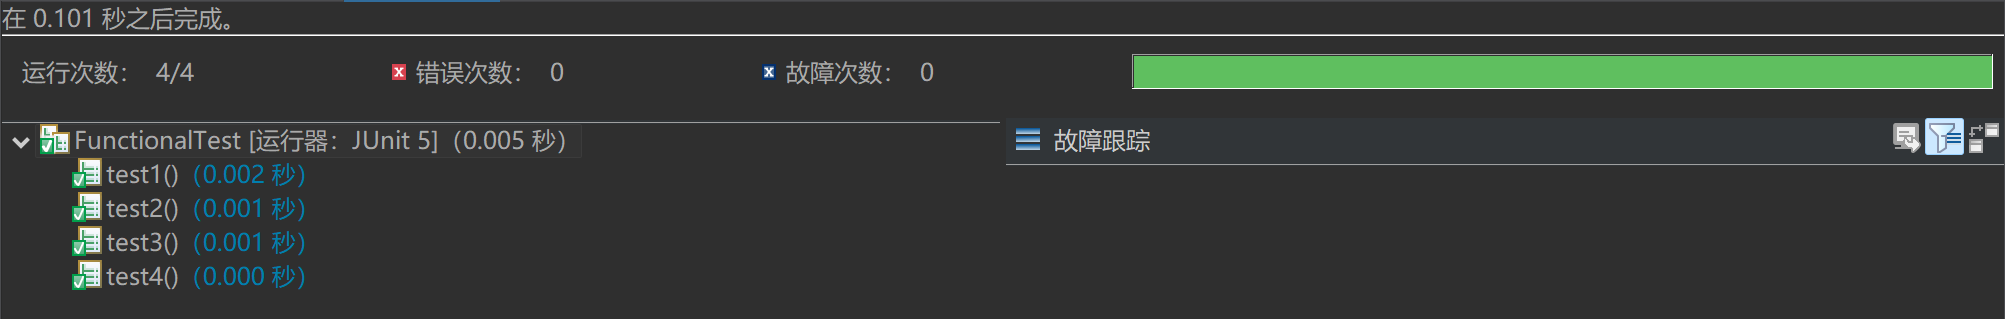
\includegraphics[width=0.8\linewidth]{figure/FunctionalTest.png}
        \caption{功能测试结果示意图}
    \end{figure}

    综上所述,功能性测试的通过验证了当前版本语法分析器在正确性与健壮性方面具备良好的表现,能够满足对中缀表达式转换为后缀表达式的核心功能需求。该测试为后续性能评估与多线程并发测试奠定了坚实基础。此部分的测试案例可见\ \textit{附录B:功能测试案例清单}。

    \subsection{比较静态成员与非静态成员}

    在本实验所构建的表达式语法分析器中,\verb|lookahead| 变量的设计选择对系统的可并发性与运行稳定性具有关键影响。\verb|lookahead| 作为语法分析过程中核心的输入符号读取指针,其作用是维护分析器对当前输入状态的追踪与判断。在最初实现中,\verb|lookahead| 被定义为类的静态成员变量。这一设计在单线程环境下通常不会引发功能性问题,且在性能表现上差异甚微,故而不易引起注意。

    然而,随着实验扩展至并发测试场景,即在多线程环境中对多个表达式并行解析时,\verb|lookahead| 作为静态变量的弊端便显现无遗。由于静态成员在Java中属于类级别的存储区域,所有该类的实例将共享同一份静态变量。这种共享特性意味着,不同线程中构造的多个 \verb|Parser| 实例会操作同一个 \verb|lookahead| 实例,从而导致“串扰”(interference)现象,即一个线程尚未完成的输入处理会被另一个线程无意间覆盖,进而引起语法状态判断错误。这种状态冲突会导致即便输入字符串本身完全合法,也可能因 \verb|lookahead| 值在多线程中被提前修改而被误判为非法表达式。

    为验证这一问题,本实验设置了多线程的并发解析测试。每个线程负责生成并解析一串长度递增的合法表达式字符串。在静态成员变量版本的测试中,多个线程频繁出现语法分析失败的情况,表明系统未能正确解析结构完全合法的表达式,表现出明显的线程间干扰。而当将 \verb|lookahead| 重构为非静态成员变量后,各个 \verb|Parser| 实例维护独立的输入读取状态,不再共享相同的符号指针,各线程得以在互不影响的环境中完成语法解析任务。经对比实验确认,所有合法表达式均可被准确识别,线程之间的语义冲突问题完全消除。

    \begin{figure}[htbp]
        \centering
        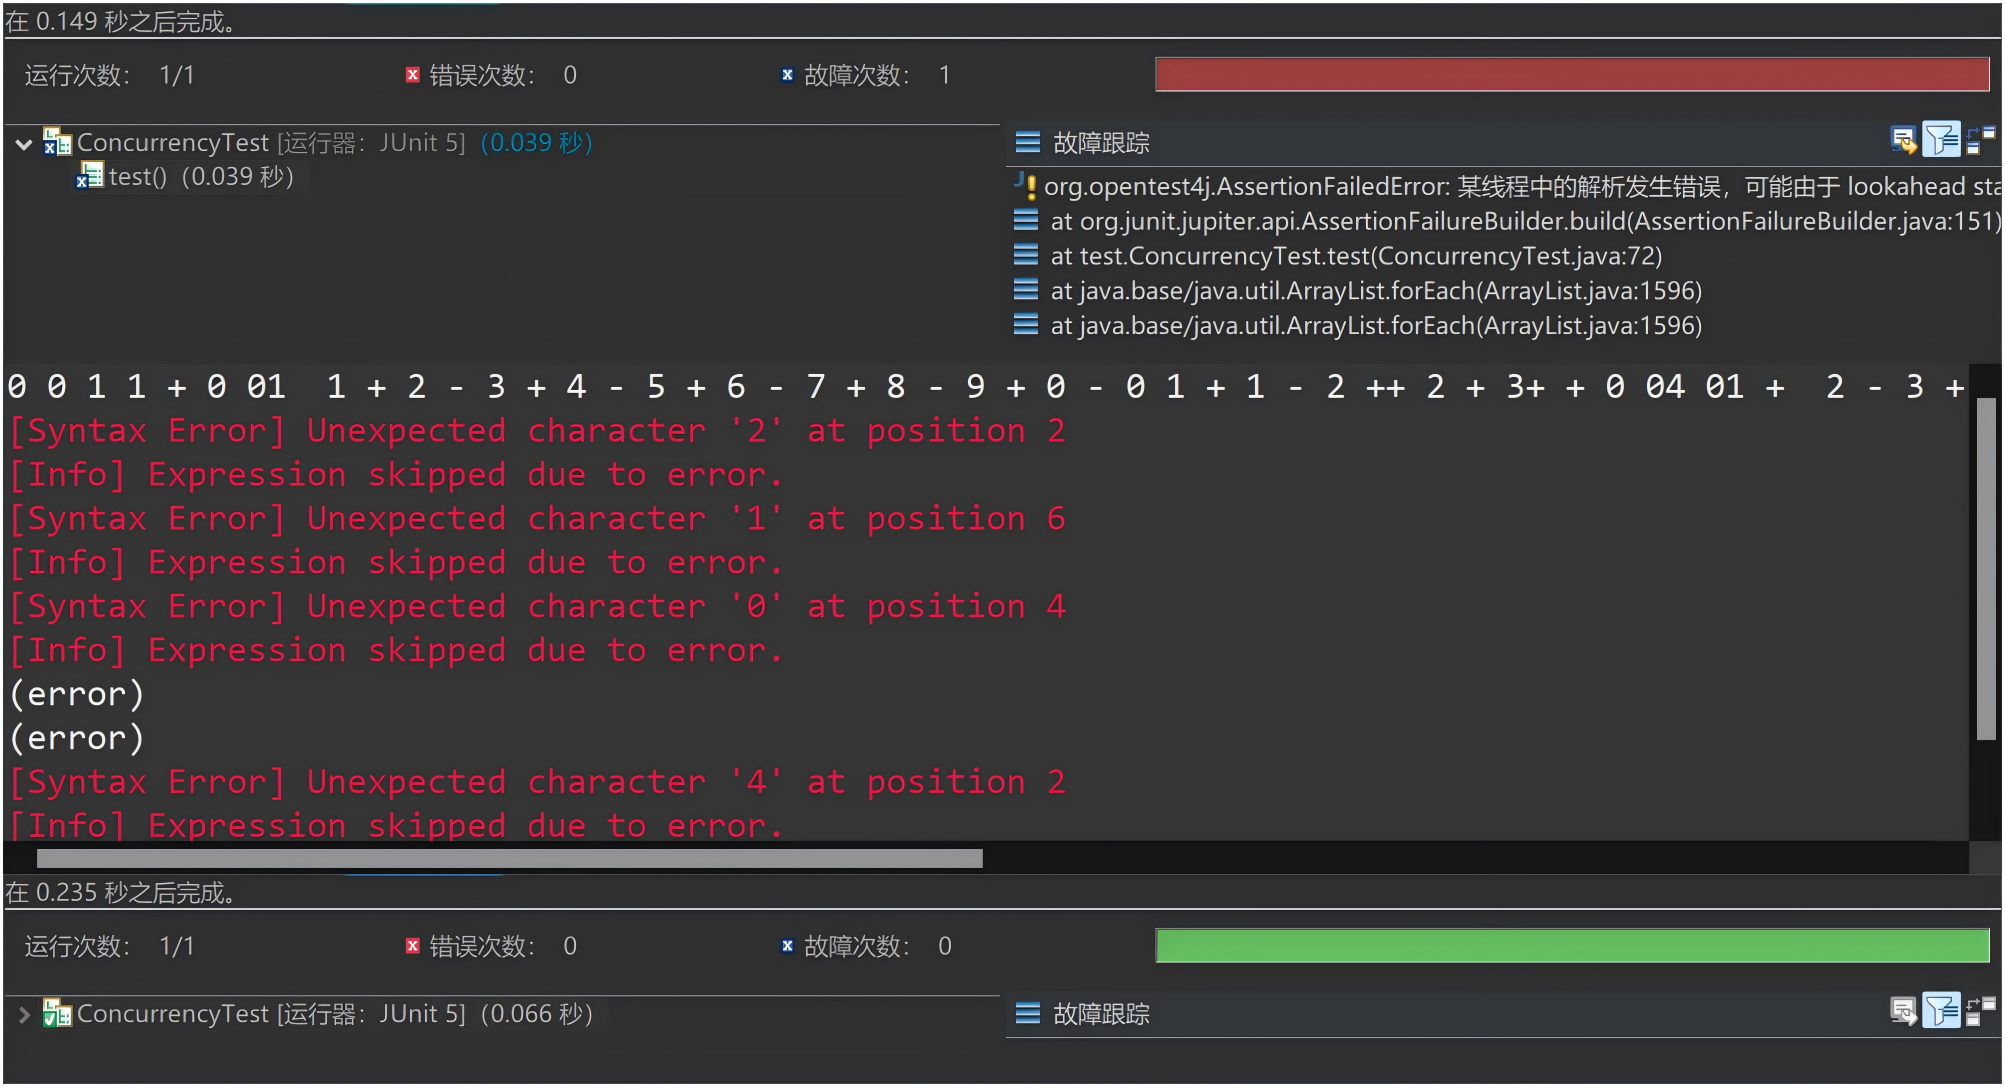
\includegraphics[width=0.8\linewidth]{figure/ConcurrencyTest.png}
        \caption{静态测试结果示意图}
    \end{figure}

    由此可见,在并发编译场景下,对于状态变量如 \verb|lookahead| 的设计必须避免采用静态成员结构,以保证语法分析器的线程安全性和正确性。静态成员虽然在某些特定情形下可提升共享效率,但其在多线程语境中的副作用亦不可忽视。该部分实验清晰地揭示了静态与非静态成员在语法分析模块中行为表现的本质差异,对提升语法分析器的健壮性具有重要启示意义。此部分的测试案例可见\ \textit{附录C:静态测试源程序清单}。

    \subsection{比较消除尾递归前后程序的性能}

    在本实验的比较消除尾递归前后程序性能部分,重点对比分析了两种语法解析器实现方案的性能表现:一种采用传统递归调用的方式实现表达式语法分析(RecursionParser),另一种则使用消除尾递归后基于循环实现的语法分析器。测试通过构造长度从1到10001逐步递增的解析表达式,系统性地测量每种实现处理相应输入时的平均运行时间,从而全面评估尾递归优化对实际编译器前端性能的影响。

    实验使用了程序自动生成的表达式样本,每组样本在测试中重复运行十次以获取更稳定的平均时间结果,并对不同输入长度下的运行时间进行记录与对比。结果通过控制变量法排除了系统输出等干扰因素,并采用标准的纳秒级计时方式,确保实验数据的准确性和可比性。

    \begin{figure}[htbp]
        \centering
        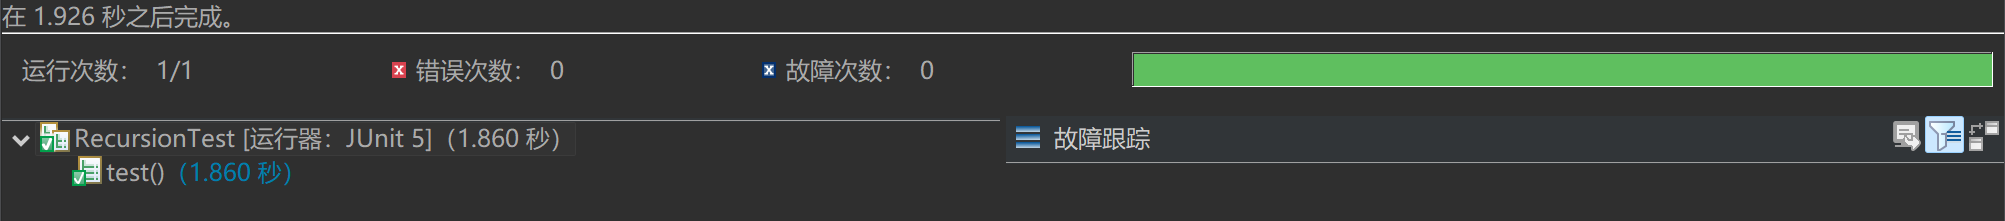
\includegraphics[width=0.8\linewidth]{figure/RecursionTest.png}
        \caption{递归测试结果示意图}
    \end{figure}
    
    从测试数据来看,两种解析器在小规模输入(长度不超过几百)时的运行时间几乎没有显著差异,甚至部分情况下递归版本略优于循环版本。这一结果初看似乎违背了尾递归优化预期提升性能的结论。然而深入分析可以发现,这种表现主要源于 Java 虚拟机(JVM)在编译阶段对尾递归调用的自动优化。由于 JVM 能够在一定程度上识别尾调用并进行优化处理,递归形式在实际运行时并未带来显著的性能开销。因此在某些场景下,递归版本反而可能因为更简单直接的调用路径而表现更优。
    
    随着输入表达式长度的持续增长,循环版本逐渐在总体趋势上表现出更为稳定和略优的性能表现。尤其在大于 5000 的表达式长度测试中,虽然两者差距仍较小,但可以观察到递归实现的波动性略高,部分数据点存在突发的运行时间上升,这可能与 JVM 栈空间资源调度有关。相比之下,循环版本在处理超大输入时保持了更好的时间稳定性和资源控制能力。

    \begin{figure}[htbp]
        \centering
        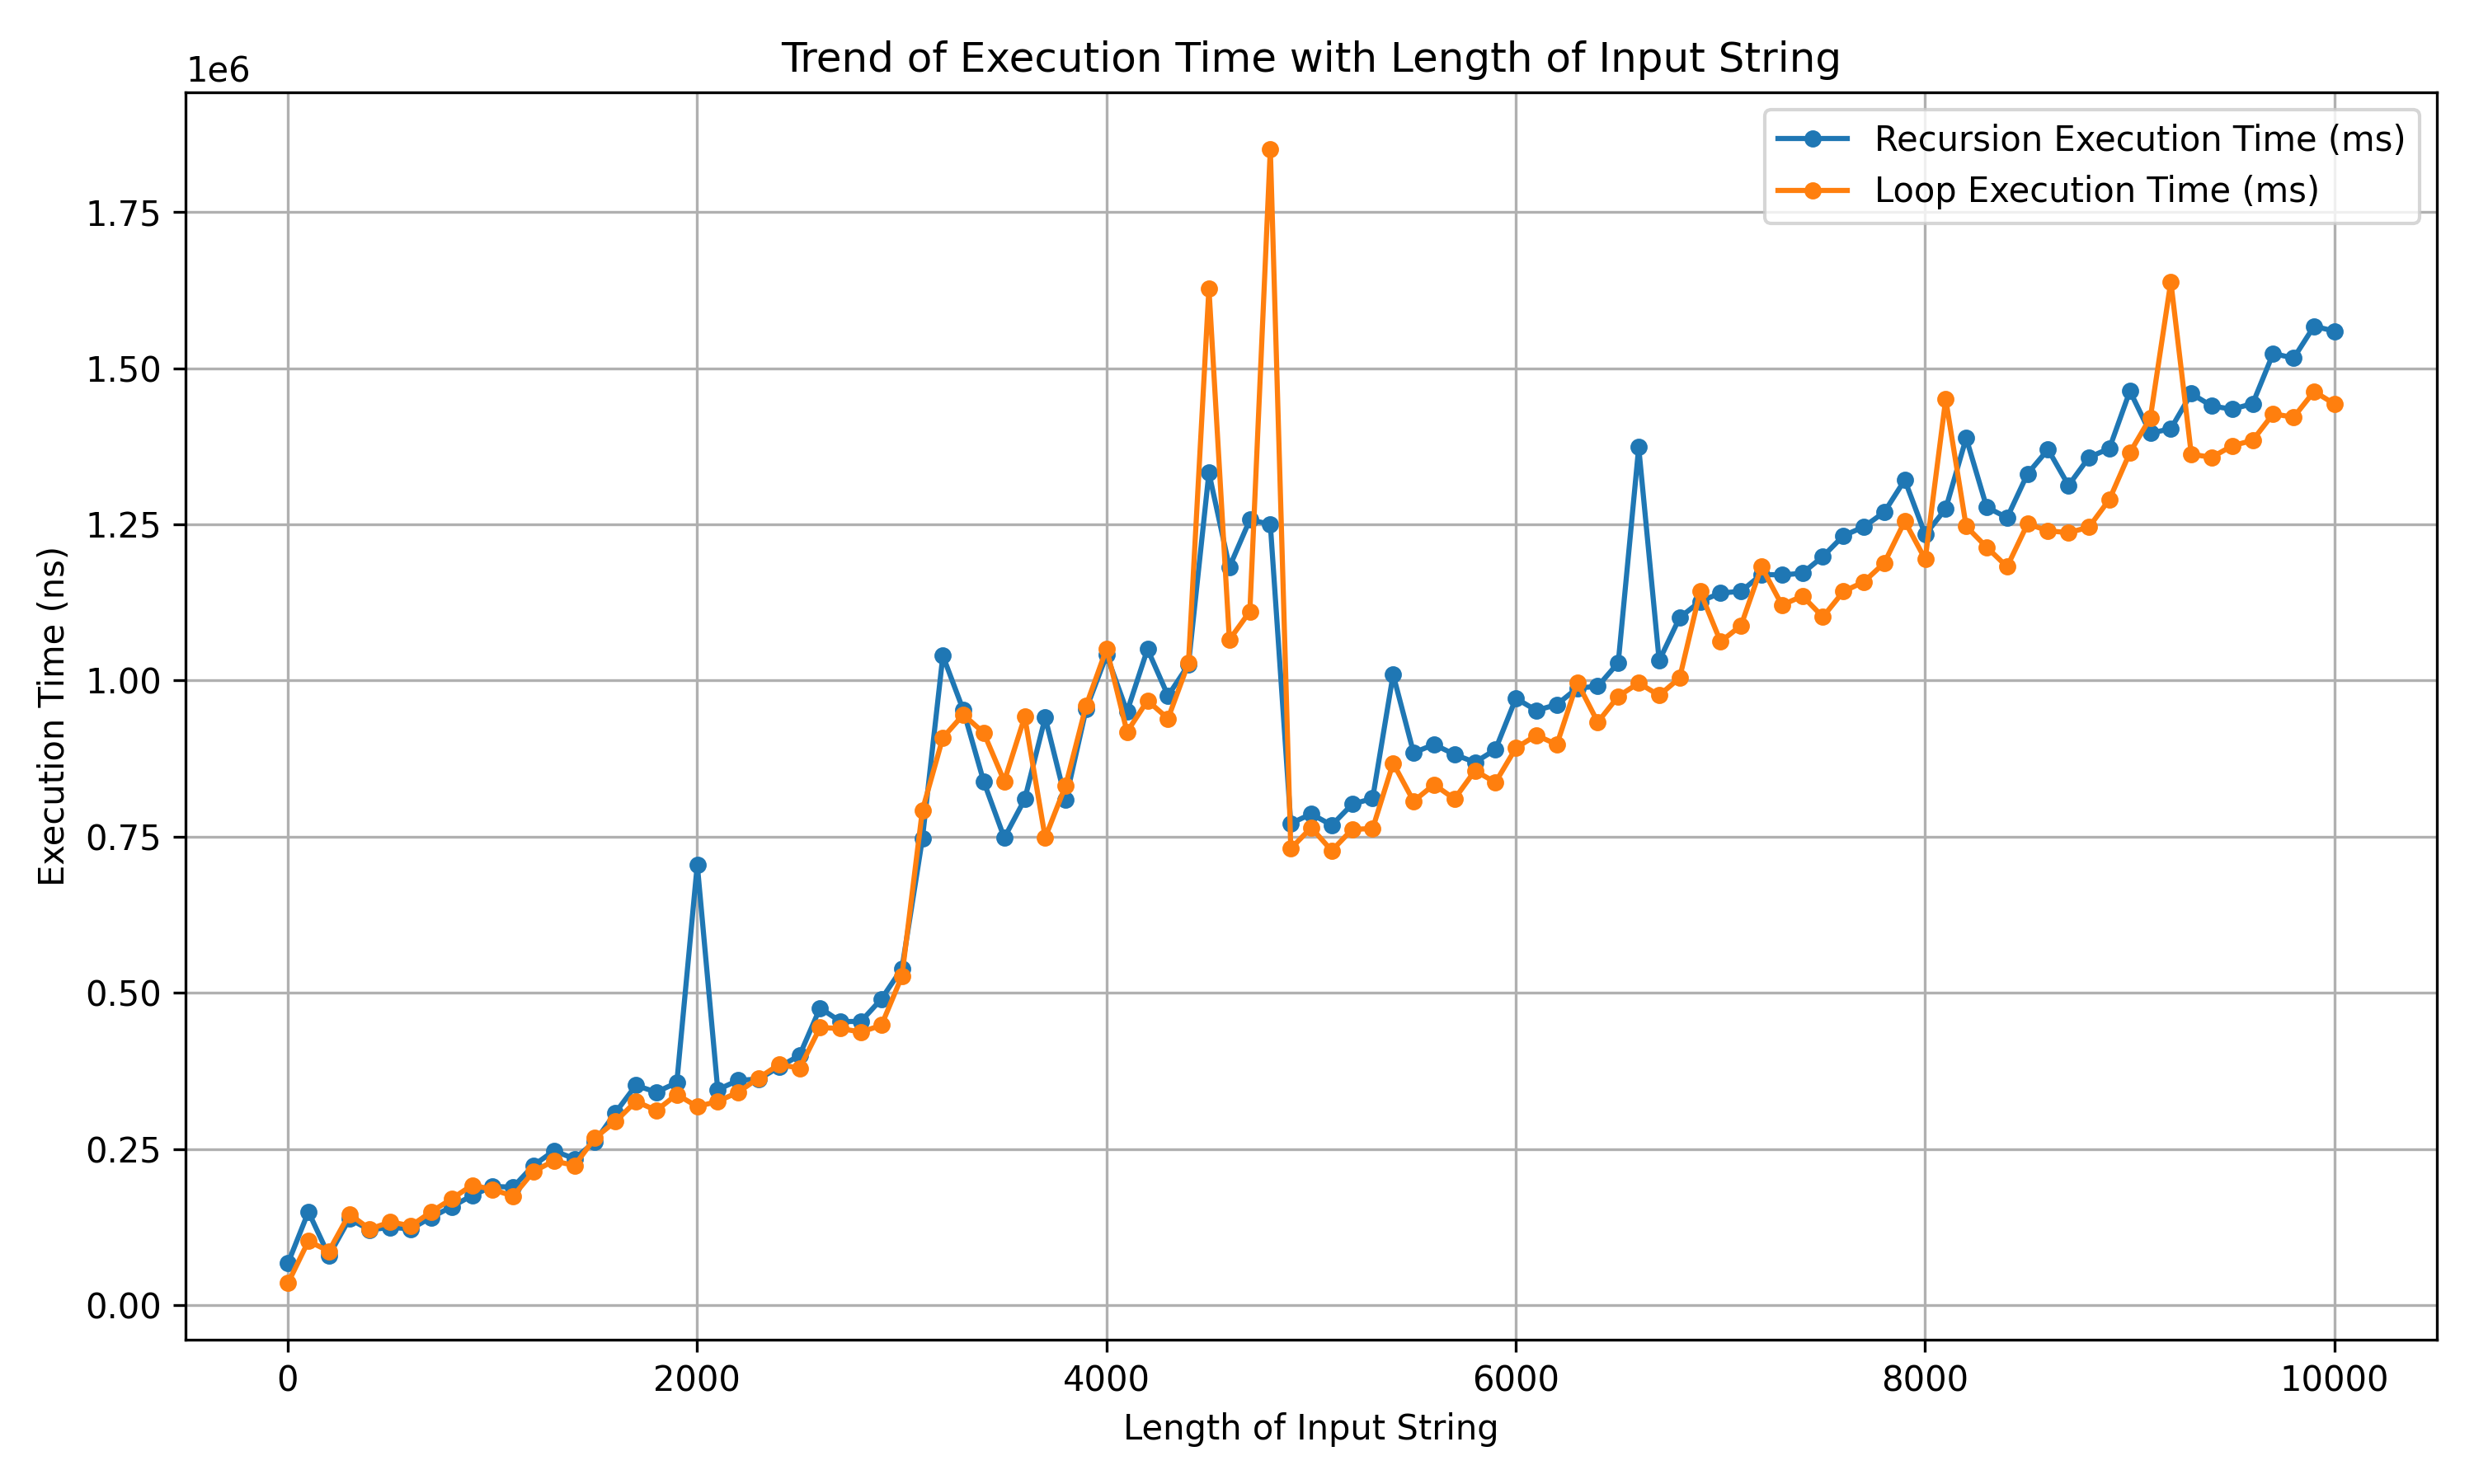
\includegraphics[width=0.5\linewidth]{figure/TimeTrend.png}
        \caption{递归测试时间趋势图}
    \end{figure}
    
    综上所述,本实验通过系统性地测试和对比尾递归与循环实现的表达式语法分析器性能,验证了在现代 Java 编译器优化机制下,尾递归的性能劣势已被大幅削弱。但从整体上来看,消除尾递归后的循环版本在处理长表达式时仍具有略优的稳定性与效率,特别适合用于对性能要求较高的编译器构造实践项目。此测试不仅验证了尾递归优化的理论意义,也进一步强化了对编译器优化行为在实际程序执行中表现的理解。此部分的测试案例可见\ \textit{附录D:递归测试源程序清单}。此部分的测试结果可见\ \textit{附录F:递归测试原始数据}

    \subsection{扩展错误处理功能}

    在本次实验中,为增强后缀表达式转换程序的健壮性与实用性,扩展错误处理功能成为关键的设计目标之一。为了系统性地评估该功能的有效性,设计了四种具有代表性的输入错误场景,分别测试程序在面对非法字符、表达式结构不完整、运算符混乱、以及输入格式不规范等情况下的表现。每个测试用例均采用 JUnit 编写,输入通过 \verb|ByteArrayInputStream| 模拟,输出结果通过重定向 \verb|System.out| 至 \verb|ByteArrayOutputStream| 实现截取,并与预期的错误提示进行比对,从而验证解析器的容错能力。

    \begin{figure}[htbp]
        \centering
        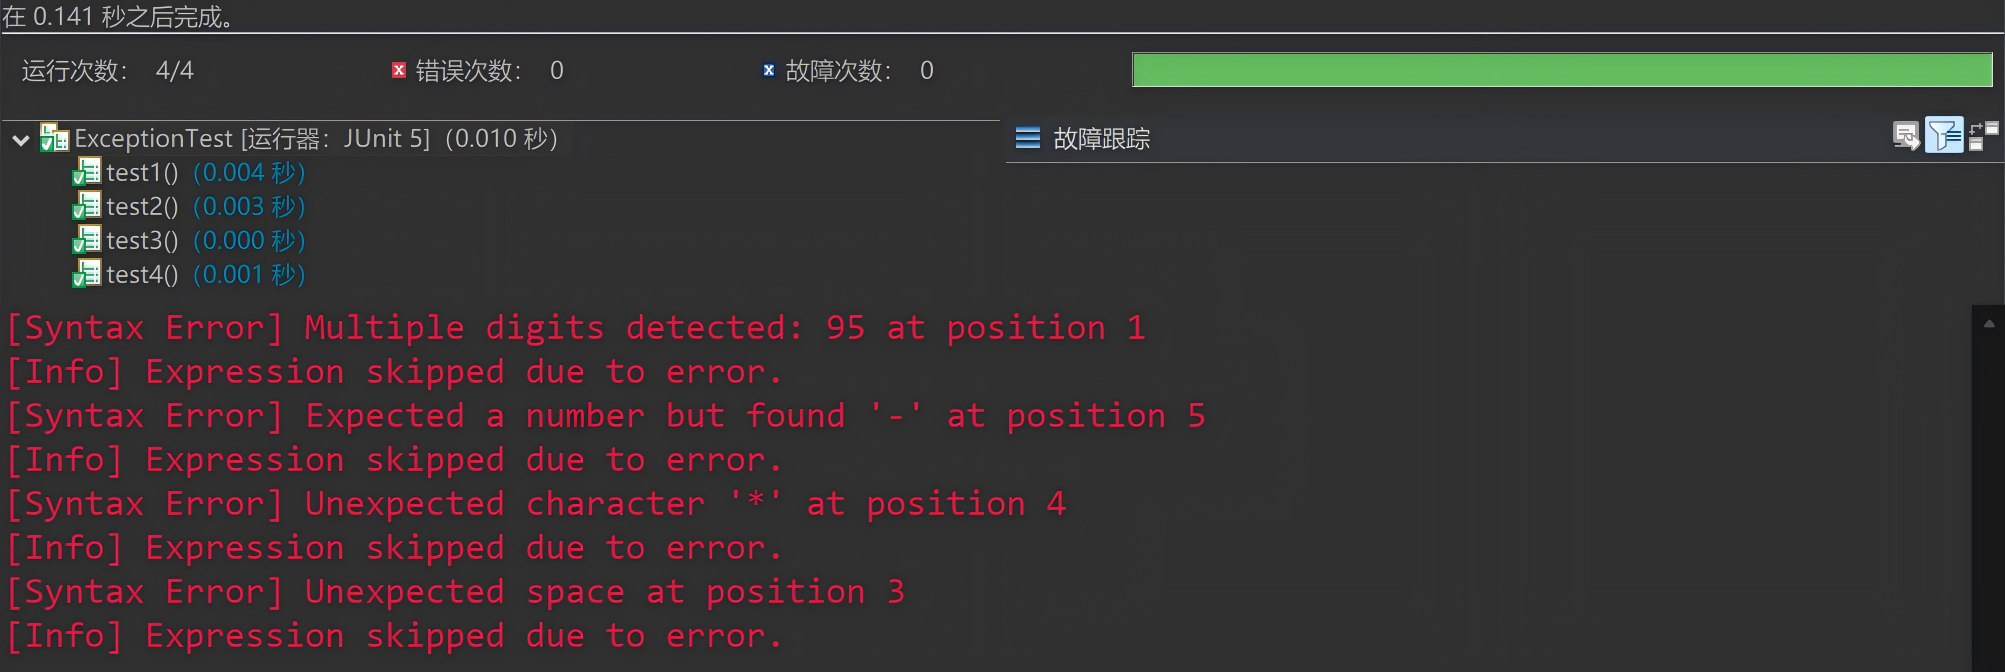
\includegraphics[width=0.8\linewidth]{figure/ExceptionTest.png}
        \caption{异常测试结果示意图}
    \end{figure}

    测试结果显示,程序能够准确检测输入表达式中的不同类型错误,并在输出结果中标注错误发生的位置,同时保留当前已处理的表达式部分,从而为用户提供清晰直观的错误提示。例如,测试用例中表达式 “$95+2$” 中由于缺乏运算符间的操作数分隔,程序成功地标识出非法字符 ‘$5$’ 紧接在 ‘$9$’ 之后的错误,并输出 “\verb|9 (error)|”。而对于表达式 “$9-5+-2$”,程序能够捕捉到连续运算符 $+$ 和 $-$ 所引发的语法混乱,并准确地中止在错误位置前输出 “\verb|9 5 - (error)|”,提示用户运算表达式结构的错误。此外,对于表达式 “$9-5*2+6$”,尽管其结构在数学语义上是合法的,但由于当前语法规则未覆盖乘法操作符,解析器也能识别出超出支持范围的符号,提供一致的错误报告。
    
    通过以上扩展性测试可以看出,程序的错误处理机制不仅能检测常见的语法错误,而且在输出中明确标示错误发生的位置,增强了对使用者的交互友好性。在实际使用场景中,该功能对于初学者理解表达式构造规则、定位输入错误具有显著的指导意义,从而提升了整个编译器前端模块的健壮性和可维护性。整体而言,本实验在语法分析器中融入扩展错误处理逻辑的尝试是成功的,也为后续更复杂语法支持与容错机制的引入奠定了良好基础。此部分的测试案例可见\ \textit{附录E:异常测试案例清单}。

    \section{总结与展望}

    \subsection{实验总结}

    本次实验围绕中缀表达式转换为后缀表达式的简易编译器前端进行了系统性的结构优化与功能增强。在实验实施过程中,通过将原程序中使用的静态成员变量重构为非静态形式,有效改善了状态管理的灵活性与程序复用性。尾递归的成功消除进一步提升了解析过程的运行效率,显著降低了程序在处理长表达式时的栈消耗与栈溢出风险。在健壮性方面,实验实现了对非法输入的识别与分类报错机制,使程序具备了基本的错误提示能力,有助于提升交互体验与系统容错性。此外,Javadoc 注释与文档的生成规范了程序的文档化流程,JUnit 测试的引入亦增强了对各功能模块稳定性和正确性的验证手段。总体而言,实验在语法制导翻译的基础上,成功实现了语法分析器的结构优化、性能提升与容错扩展,为构建更完善的语法处理系统打下了良好基础。

    \subsection{未来展望}

    尽管实验已实现基本功能的完善与部分性能的优化,但其仍存在进一步扩展的潜力。首先,当前的语法分析器仅支持数字常量与加减运算,未来可考虑引入多位数处理、括号优先级规则及扩展乘除等运算符,从而支持更复杂的表达式结构。此外,在错误处理方面,可探索更加细粒度的错误恢复机制,实现语法错误的自动同步与上下文恢复,使分析器具备更强的健壮性与交互容忍度。在程序结构层面,引入基于 LL(1) 或 LR(1) 分析技术的自动语法分析表驱动方法,有望取代手工递归下降过程,进一步提升通用性与可维护性。实验过程中所培养的文档化、模块化与测试意识,对后续课程如词法分析器生成、语义翻译及中间代码生成等实验任务的完成具有重要参考价值,也为更深入理解编译器体系结构与实现机制提供了坚实支撑。随着后续实验的开展,此次实验积累的编码实践经验与语法分析理论知识将发挥持续作用,助力构建完整的编译器前端。
	
    \addcontentsline{toc}{section}{参考文献}
    \begin{thebibliography}{99}
        \bibitem{ref1} 沐言科技\ 李兴华.\ Java编程\ 从入门到实践[M].\ 第1版.\ 安徽:中国水利水电出版社,\ 2021.
        \bibitem{ref2} Aho\ A\ V,\ SLam\ M,\ Sethi\ R,\ etal.\ 编译原理[M].\ 赵建华\ 等译.\ 第2版.\ 北京:机械工业出版社,\ 2009.
        \bibitem{ref3} LI\ W\ J.\ Lecture04:\ Top\ Down\ Parsing[PPT][Z].\ Sun\ Yat-sen\ University,\ 2022.
    \end{thebibliography}
	
	\newpage
	\appendix
	\centerline{\Large{\textbf{附录}}}

    \section{原始源程序清单}

    \begin{minted}[baselinestretch=1, framesep=2mm, escapeinside=||]{java}
import java.io.*;

class Parser {
    static int lookahead;

    public Parser() throws IOException {
        lookahead = System.in.read();
    }

    void expr() throws IOException {
        term();
        rest();
    }

    void rest() throws IOException {
        if (lookahead == '+') {
            match('+');
            term();
            System.out.write('+');
            rest();
        } else if (lookahead == '-') {
            match('-');
            term();
            System.out.write('-');
            rest();
        } else {
            // do nothing with the input
        }
    }

    void term() throws IOException {
        if (Character.isDigit((char)lookahead)) {
            System.out.write((char)lookahead);
            match(lookahead);
        } else  throw new Error("syntax error");
    }

    void match(int t) throws IOException {
        if (lookahead == t)  lookahead = System.in.read();
        else  throw new Error("syntax error");
    }
}

public class Postfix {
    public static void main(String[] args) throws IOException {
        System.out.println("Input an infix expression and output its postfix
    notation:");
        new Parser().expr();
        System.out.println("\nEnd of program.");
    }
}
    \end{minted}

    \section{功能测试案例清单}

    \begin{minted}[baselinestretch=1, framesep=2mm, escapeinside=||]{java}
class FunctionalTest {

    @Test
    void test1() throws IOException {
        String line = "1+1";

        ByteArrayOutputStream buffer = new ByteArrayOutputStream();
        PrintStream originalOut = System.out;
        System.setOut(new PrintStream(buffer));

        ByteArrayInputStream input = new ByteArrayInputStream(line.getBytes());
        Parser parser = new Parser(input);
        // RecursionParser parser = new RecursionParser(input);
        parser.expr();

        System.setOut(originalOut);
        String result = buffer.toString().trim();
        assertEquals("1 1 +", result);
    }

    @Test
    void test2() throws IOException {
        String line = "9-5+2";

        ByteArrayOutputStream buffer = new ByteArrayOutputStream();
        PrintStream originalOut = System.out;
        System.setOut(new PrintStream(buffer));

        ByteArrayInputStream input = new ByteArrayInputStream(line.getBytes());
        Parser parser = new Parser(input);
        // RecursionParser parser = new RecursionParser(input);
        parser.expr();

        System.setOut(originalOut);
        String result = buffer.toString().trim();
        assertEquals("9 5 - 2 +", result);
    }

    @Test
    void test3() throws IOException {
        String line = "1+2+3+4+5";

        ByteArrayOutputStream buffer = new ByteArrayOutputStream();
        PrintStream originalOut = System.out;
        System.setOut(new PrintStream(buffer));

        ByteArrayInputStream input = new ByteArrayInputStream(line.getBytes());
        Parser parser = new Parser(input);
        // RecursionParser parser = new RecursionParser(input);
        parser.expr();

        System.setOut(originalOut);
        String result = buffer.toString().trim();
        assertEquals("1 2 + 3 + 4 + 5 +", result);
    }

    @Test
    void test4() throws IOException {
        String line = "1-2+3-4+5-6+7-8+9-0";

        ByteArrayOutputStream buffer = new ByteArrayOutputStream();
        PrintStream originalOut = System.out;
        System.setOut(new PrintStream(buffer));

        ByteArrayInputStream input = new ByteArrayInputStream(line.getBytes());
        Parser parser = new Parser(input);
        // RecursionParser parser = new RecursionParser(input);
        parser.expr();

        System.setOut(originalOut);
        String result = buffer.toString().trim();
        assertEquals("1 2 - 3 + 4 - 5 + 6 - 7 + 8 - 9 + 0 -", result);
    }
}
    \end{minted}

    \section{静态测试源程序清单}

    \begin{minted}[baselinestretch=1, framesep=2mm, escapeinside=||]{java}
class ConcurrencyTest {

    static class ParseTask implements Callable<Boolean> {
    
        private final String expression;

        public ParseTask(String expression) {
            this.expression = expression;
        }

        @Override
        public Boolean call() {
            try {
                InputStream input = new ByteArrayInputStream(expression.getBytes());

                Parser parser = new Parser(input);
                parser.expr();

                return !parser.hadError();
            } catch (Exception e) {
                return false;
            }
        }
    }

    private static String generateExpression(int length) {
        StringBuilder sb = new StringBuilder();
        for (int i = 0; i < length; i++) {
            sb.append(i % 10);
            if (i != length - 1) {
                sb.append(i % 2 == 0 ? '+' : '-');
            }
        }
        return sb.toString();
    }

    @Test
    void test() throws InterruptedException {
        int threadCount = 10;
        ExecutorService executor = Executors.newFixedThreadPool(threadCount);
        List<Future<Boolean>> results = new ArrayList<>();

        for (int i = 0; i < threadCount; i++) {
            String expr = generateExpression(10 + i);
            results.add(executor.submit(new ParseTask(expr)));
        }

        executor.shutdown();

        boolean finished = executor.awaitTermination(10, TimeUnit.SECONDS);
        assertTrue(finished, "线程可能陷入死锁");

        for (Future<Boolean> future : results) {
            try {
                assertTrue(future.get(), "某线程中的解析发生错误,可能由于 lookahead"
                                       + "static 导致串扰");
            } catch (ExecutionException e) {
                fail("解析线程抛出异常:" + e.getCause().getMessage());
            }
        }
    }
}
    \end{minted}

    \section{递归测试源程序清单}

    \begin{minted}[baselinestretch=1, framesep=2mm, escapeinside=||]{java}
class RecursionTest {

    private static String generateExpression(int length) {
        StringBuilder sb = new StringBuilder();
        for (int i = 0; i < length; i++) {
            sb.append(i % 10);
            if (i != length - 1) {
                sb.append(i % 2 == 0 ? '+' : '-');
            }
        }
        return sb.toString();
    }

    private static long measureParserTime(String inputStr, boolean useRecursion)
    throws IOException {
        ByteArrayInputStream input = new ByteArrayInputStream(inputStr.getBytes());
        ByteArrayOutputStream buffer = new ByteArrayOutputStream();
        PrintStream originalOut = System.out;

        System.setOut(new PrintStream(buffer));
        long start = System.nanoTime();
        
        try {
            if (useRecursion) {
                RecursionParser parser = new RecursionParser(input);
                parser.expr();
            } else {
                Parser parser = new Parser(input);
                parser.expr();
            }
        } catch (Exception e) {
            System.setOut(originalOut);
            System.err.println("Exception occurred in " +
            (useRecursion ? "RecursionParser" : "Parser") +
            ": " + e.getMessage());
            e.printStackTrace();
            return -1;
        }

        long end = System.nanoTime();
        System.setOut(originalOut);
        return (end - start);
    }

    @Test
    void test() throws IOException {
        System.out.println("Length\tRecursion(ns)\tLoop(ns)");
        long startTime = System.currentTimeMillis();
        
        for (int length = 1; length <= 10001; length += 100) {
            String expr = generateExpression(length);
            long totalRec = 0, totalLoop = 0;
            int repeat = 10;

            for (int i = 0; i < repeat; i++) {
                totalRec += measureParserTime(expr, true);
                totalLoop += measureParserTime(expr, false);
            }

            long avgRec = totalRec / repeat;
            long avgLoop = totalLoop / repeat;
            System.out.println(length + "\t" + avgRec + "\t\t" + avgLoop);
        }
        
        long duration = System.currentTimeMillis() - startTime;
        assertTrue(duration < 3000, "表达式处理时间超出预期!");
    }
}
    \end{minted}

    \section{异常测试案例清单}

    \begin{minted}[baselinestretch=1, framesep=2mm, escapeinside=||]{java}
class ExceptionTest {

    @Test
    void test1() throws IOException {
        String line = "95+2";

        ByteArrayOutputStream buffer = new ByteArrayOutputStream();
        PrintStream originalOut = System.out;
        System.setOut(new PrintStream(buffer));

        ByteArrayInputStream input = new ByteArrayInputStream(line.getBytes());
        Parser parser = new Parser(input);
        // RecursionParser parser = new RecursionParser(input);
        parser.expr();

        System.setOut(originalOut);
        String result = buffer.toString().trim();
        assertEquals("9 (error)", result);
    }

    @Test
    void test2() throws IOException {
        String line = "9-5+-2";

        ByteArrayOutputStream buffer = new ByteArrayOutputStream();
        PrintStream originalOut = System.out;
        System.setOut(new PrintStream(buffer));

        ByteArrayInputStream input = new ByteArrayInputStream(line.getBytes());
        Parser parser = new Parser(input);
        // RecursionParser parser = new RecursionParser(input);
        parser.expr();

        System.setOut(originalOut);
        String result = buffer.toString().trim();
        assertEquals("9 5 - (error)", result);
    }

    @Test
    void test3() throws IOException {
        String line = "9-5*2+6";

        ByteArrayOutputStream buffer = new ByteArrayOutputStream();
        PrintStream originalOut = System.out;
        System.setOut(new PrintStream(buffer));

        ByteArrayInputStream input = new ByteArrayInputStream(line.getBytes());
        Parser parser = new Parser(input);
        // RecursionParser parser = new RecursionParser(input);
        parser.expr();

        System.setOut(originalOut);
        String result = buffer.toString().trim();
        assertEquals("9 5 - (error)", result);
    }

    @Test
    void test4() throws IOException {
        String line = "9- 5+2";

        ByteArrayOutputStream buffer = new ByteArrayOutputStream();
        PrintStream originalOut = System.out;
        System.setOut(new PrintStream(buffer));

        ByteArrayInputStream input = new ByteArrayInputStream(line.getBytes());
        Parser parser = new Parser(input);
        // RecursionParser parser = new RecursionParser(input);
        parser.expr();

        System.setOut(originalOut);
        String result = buffer.toString().trim();
        assertEquals("9 (error)", result);
    }
}
    \end{minted}

    \section{递归测试原始数据}

    	\begin{center}
	    \setlength{\LTcapwidth}{\textwidth}
	    \small
	    
	    \begin{longtable}{
	        >{\centering\arraybackslash}m{.09\textwidth}
	        | >{\centering\arraybackslash}m{.09\textwidth}
	      | >{\centering\arraybackslash}m{.09\textwidth}
	        || >{\centering\arraybackslash}m{.09\textwidth}
	      | >{\centering\arraybackslash}m{.09\textwidth}
	        | >{\centering\arraybackslash}m{.09\textwidth}
	      || >{\centering\arraybackslash}m{.09\textwidth}
	        | >{\centering\arraybackslash}m{.09\textwidth}
	      | >{\centering\arraybackslash}m{.09\textwidth}
	    }
	        
	        \toprule
	        \textbf{数组长度} & \textbf{递归版本(ns)} & \textbf{循环版本(ns)} & \textbf{数组长度} & \textbf{递归版本(ns)} & \textbf{循环版本(ns)} & \textbf{数组长度} & \textbf{递归版本(ns)} & \textbf{循环版本(ns)} \\
	        \midrule
	        \endfirsthead
	        
	        \multicolumn{9}{c}{\footnotesize 续表} \\
	        \toprule
	        \textbf{数组长度} & \textbf{递归版本(ns)} & \textbf{循环版本(ns)} & \textbf{数组长度} & \textbf{递归版本(ns)} & \textbf{循环版本(ns)} & \textbf{数组长度} & \textbf{递归版本(ns)} & \textbf{循环版本(ns)} \\
	        \midrule
	        \endhead
	        
	        \midrule
	        \multicolumn{9}{r}{\footnotesize 接下页} \\
	        \endfoot
	        
	        \bottomrule
	        \endlastfoot
	        
	        1 & 67079 & 35290 & 3401 & 837989 & 916190 & 6801 & 1100780 & 1004210 \\
            101 & 149619 & 102610 & 3501 & 748190 & 838910 & 6901 & 1126660 & 1142610 \\
            201 & 79200 & 86570 & 3601 & 809910 & 941979 & 7001 & 1140179 & 1062220 \\
            301 & 138149 & 145949 & 3701 & 940819 & 748500 & 7101 & 1142850 & 1088140 \\
            401 & 120500 & 121769 & 3801 & 808869 & 832180 & 7201 & 1169910 & 1182159 \\
            501 & 124749 & 133419 & 3901 & 954220 & 960030 & 7301 & 1169109 & 1120839 \\
            601 & 122109 & 126960 & 4001 & 1040969 & 1051020 & 7401 & 1171779 & 1135320 \\
            701 & 140520 & 149449 & 4101 & 950319 & 917830 & 7501 & 1198709 & 1101920 \\
            801 & 157709 & 170249 & 4201 & 1050270 & 967949 & 7601 & 1231850 & 1142519 \\
            901 & 175660 & 192179 & 4301 & 975609 & 939150 & 7701 & 1246120 & 1158030 \\
            1001 & 190060 & 185369 & 4401 & 1025220 & 1028150 & 7801 & 1269650 & 1188260 \\
            1101 & 189059 & 174559 & 4501 & 1332770 & 1628230 & 7901 & 1321150 & 1255070 \\
            1201 & 223840 & 214060 & 4601 & 1181600 & 1065240 & 8001 & 1233609 & 1194030 \\
            1301 & 247220 & 231239 & 4701 & 1257400 & 1110699 & 8101 & 1275080 & 1450370 \\
            1401 & 234430 & 223440 & 4801 & 1250199 & 1850920 & 8201 & 1388330 & 1246819 \\
            1501 & 261880 & 267830 & 4901 & 771169 & 730979 & 8301 & 1277720 & 1213609 \\
            1601 & 308109 & 294050 & 5001 & 786569 & 764559 & 8401 & 1260730 & 1182159 \\
            1701 & 351969 & 326320 & 5101 & 768419 & 727609 & 8501 & 1331070 & 1250880 \\
            1801 & 341000 & 311800 & 5201 & 802009 & 761810 & 8601 & 1369999 & 1239770 \\
            1901 & 356380 & 337259 & 5301 & 811390 & 763069 & 8701 & 1312430 & 1236780 \\
            2001 & 705460 & 318030 & 5401 & 1009720 & 867800 & 8801 & 1357350 & 1245630 \\
            2101 & 345040 & 326260 & 5501 & 884380 & 806880 & 8901 & 1371689 & 1289980 \\
            2201 & 360100 & 340989 & 5601 & 897750 & 833500 & 9001 & 1463490 & 1364980 \\
            2301 & 361899 & 363740 & 5701 & 881720 & 810489 & 9101 & 1396040 & 1420730 \\
            2401 & 381180 & 385429 & 5801 & 869069 & 855769 & 9201 & 1403170 & 1638730 \\
            2501 & 400140 & 379410 & 5901 & 889540 & 836920 & 9301 & 1459390 & 1362249 \\
            2601 & 475900 & 444500 & 6001 & 971559 & 892119 & 9401 & 1439550 & 1357440 \\
            2701 & 454010 & 443039 & 6101 & 952090 & 912459 & 9501 & 1434439 & 1375859 \\
            2801 & 454410 & 437160 & 6201 & 961609 & 897610 & 9601 & 1443370 & 1384609 \\
            2901 & 490300 & 448270 & 6301 & 988000 & 997160 & 9701 & 1523700 & 1427029 \\
            3001 & 538930 & 526670 & 6401 & 990789 & 933339 & 9801 & 1516130 & 1421560 \\
            3101 & 746760 & 792470 & 6501 & 1028569 & 974829 & 9901 & 1567379 & 1462849 \\
            3201 & 1039809 & 908580 & 6601 & 1373509 & 996020 & 10001 & 1559299 & 1442729 \\
            3301 & 952470 & 945499 & 6701 & 1031810 & 976320 &  &  & \\
	        
	    \end{longtable}
	    \vspace{-3em}
	\end{center}
	
\end{document}
